\chapter{Developing the Hardware} % Main chapter title

\label{Chapter4} % Change X to a consecutive number; for referencing this chapter elsewhere, use \ref{ChapterX}

There are a lot of factors that go into designing and building an electrical system that fits the needs for this project.
This process begins by outlining the requirements in Section \ref{sec:HardwareRequirements}, followed by describing the process and methodology of choosing parts in Section \ref{sec:ChoosingParts}.
Then, the feasibility of prototyping such as system is discussed in Section \ref{sec:Prototyping}, and finally the system is designed and manufactured in Sections \ref{sec:DesigningThePCB} and \ref{sec:ManufacturingThePCB} respectively.

\section{Requirements}\label{sec:HardwareRequirements}

This section will explain the different constraints taken into account while developing the hardware portion of this project.
First, the hardware must be performant enough to provide a positive user experience (\ref{subsec:HardwarePerformance}), and secondly the product must be cheap enough to justify it over similar alternatives (\ref{subsec:HardwareCost}).

\subsection{Performance}\label{subsec:HardwarePerformance}

When considering how much power needs to be incorporated in to the miniature computer, it is important to consider a number of factors, such as: having enough power to stream audio and video over the internet, not consuming too much power so as to require an expensive battery, have a fast enough connection to the internet to deliver data with the least possible latency, and having a reasonable footprint to be used as a mobile device.

Immediately, the device must be capable of decoding and rendering video that is streamed over the internet.
Such video processing is a relatively expensive process that cannot easily be done with something such as a micro controller or even a single core CPU seen on Single Board Computers (SBC) such as the Raspberry Pi Zero due to the lack of working memory and processing power \cite{picockpit_2021}.
Though at the same time, it is important to not simply build a powerful system akin to a laptop that will consume more power.
It makes no sense to built a powerful mini-computer when all it will ever be used to is to connect to another computer, and the added power draw would require a larger battery in order to stay operational for decent periods of time.
Instead it should be cut down and distilled into something that can do it's job as efficiently as possible.

The second major performance requirement of the hardware is the ability to stream this data over the internet as quickly as possible.
Because all of the data being sent to the device is live information from the host machine, the video and audio streams cannot simply be buffered in advance and played when it's ready like a recorded video.
Instead, the data must be displayed as it is received so that the user can have a smooth experience without having to wait for their keystrokes or mouse movements to be registered.
While Wi-Fi is growing ever quicker and more reliable, and should absolutely be included as a way to connected to the internet, the best way to ensure a stable and speedy connection is to use an Ethernet Cable.
This will help the device work on a consistent connection when used at a desk, while also providing a way to connect while on-the-go.

This leads to the desire for a portable design that can be used both in a conducive environnement such as a desk or while mobile.
The hardware should have the ability to be powered by a chord plugging into the device, or by an internal battery.
This alone presents a number of difficult concerns which will be addressed in Section \ref{sec:Prototyping}.
Such a requirement leads to a clear benefit of integrating crucial computers such as a battery and a screen into the hardware design, while leaving as many ports open such as ethernet and USB for the user to take advantage of.


\subsection{Cost}\label{subsec:HardwareCost}

Because this project consists of both a Hardware and Software component to make up a complete product, there must be reason for both to be developed.
While the software has the benefit of being the foundation for the connection between host and client machines, there are already hardware solutions that would theoretically be able to run such software.
Since the goal of this project is to save money by not needing to purchase an expensive mobile device to connect to a powerful desktop computer, there must be benefit in the hardware to warrant it's existence over repurposing something like an old laptop.
The most obvious metric of this is the actual cost of the hardware.
If the hardware can be produced at a high enough quality at a low enough cost to bring value over just a software solution, then it should be considered moving forward.
Otherwise it may prove that the development of the software should focus on compatibility so the hardware can be provided by the end user.

Generally speaking, the goal for the hardware of this project is to cost approximately \$100-\$200 to produce a single unit.
This comes with the understanding that hardware production in bulk often costs significantly less than assembling a single product.
The reasoning for this cost comes down to feasibility: the price of the final product should be less than what it would cost to purchase or refurbish an existing computer to do the job of this project.
Otherwise, as stated before, the software of this project may prove more valuable than the hardware as long as compatibility is kept in the forefront of development.


\section{Choosing Parts}\label{sec:ChoosingParts}

When starting to choose parts for the hardware, there are many difficult questions to face.
First and foremost, the hardware had to be built with the time and resources available for this project.
Specifically, building a Single Board Computer from scratch would be completely infeasible, but the goal was also not to simply purchase an off the shelf SBC that was not tailored to the task at hand such as a traditional Raspberry Pi.
Instead, a better suited solution would be to utilize a \emph{Raspberry Pi Compute Module 4 (CM4)} which has \enquote{The power of Raspberry Pi 4 in a compact form factor for deeply embedded applications} \cite{rpi_cm4}.
Boasting an incredibly small size and streamlined I/O, there only way to communicate with the Compute Module was through two tiny mezzanine connectors as shown in Figure \ref{fig:rpi_cm4_mezzanine}.
With no other pin outs for anything such as power, HDMI, or USB, everything had to be built on a custom Printed Circuit Board (PCB).

\begin{figure}[h]
  \centering
  \begin{minipage}{0.45\textwidth}
    \centering
    \includegraphics[width=0.9\textwidth]{Figures/rpi_cm4}
    \captionsetup{width=.75\linewidth}
    \caption[Raspberry Pi Compute Module 4]{Raspberry Pi Compute Module 4, sizing\newline55 x 40mm}
    \label{fig:rpi_cm4}
  \end{minipage}\hfill
  \begin{minipage}{0.45\textwidth}
    \centering
    \includegraphics[width=0.9\textwidth]{Figures/rpi_cm4_mezzanine}
    \captionsetup{width=.75\linewidth}
    \caption[Raspberry Pi Compute Module 4 Pin out]{Close-up of the pin out, with a 0.04mm pitch between pins}
    \label{fig:rpi_cm4_mezzanine}
  \end{minipage}
\end{figure}

This PCB would have to be designed so that the CM4 could be plugged into the board using the mezzanine connectors and rely on it for all inputs and outputs.
This, however, is only the beginning of what is required to develop the product.
Since the project would not use an off the shelf SBC like a regular Raspberry PI, the project would require only designing the PCB but also picking out all the components that would go onto the PCB, such as the USB ports themselves, the USB driver chip, and related components needed for operation.
Because the CM4 is designed to be as low-powered and compact as possible, some features that would usually be expected of such a device, like the USB ports, are disabled by default and must instead be built by the board designer.
While this helps greatly by removing extraneous components and features that aren't needed for this project, it also provides a great opportunity to learn exactly what parts are being used in the hardware.

Thought must also be given to the peripherals that will be included in the design.
Most importantly, if a screen is going to be included in the design, what kind of screen will be used?
For projects of this scale, the usual candidates for a relatively performant screen are HDMI screens or DSI screens.
While HDMI screens are much more common and recognizable, DSI screens are a new development that promises 60Hz performance in low cost and low power applications such as embedded systems.
However, when looking into existing DSI screens, there are a couple of issues that prevent it from being the best choice for this project.
Even though DSI screens are more power efficient and have built in touch support, it is a closed format which greatly restricts manufactures from producing their own screens \cite{dsi_vs_hdmi}.
Due to this, there is only one screen available for purchase outside of the official implementation, and both have a lower resolution that what is possible with HDMI screens of the same size.
So even though HDMI screens are more expensive at this size, they are a more reliable choice compared to the still-developing DSI standard.

Another potential feature to consider is whether to integrate a Real Time Clock (RTC) into the design.
An RTC is a component commonly found within laptop and desktop computers that is used to keep track of time even though the computer is powered off.
This is done with a small button battery powering an RTC chip integrated into the motherboard to keep the system's clock in sync with the real world.
While this is almost never necessary in embedded systems, it is worth considering for this project because of it's use as a mobile computer.
However, when considering the primary use case of connecting to another computer over the internet, and the potential of needing a linux kernel patch in order to add support for the RTC \cite{rtc_kernelpatch}, it would be much simpler to tell the operating system to simply resync it's clock with an internet clock every time it connects to a network.

An invaluable resource while designing the PCB was the Official I/O board for the CM4 \cite{rpi_cm4_io}.
Though the PCB board would still have to be custom built and components would need to be replaced due to the current ongoing chip shortage, it provides a great foundation instead of starting from scratch.
Another massive benefit from working within the Raspberry Pi Ecosystem is their incredible documentation and community surrounding the boards \cite{rpi_cm4_docs}.
Around the time this project was being started, the CM4 was just beginning to get into the hands of makers and developers, and only a couple custom boards had actually been made by anyone other than Raspberry Pi themselves.
Even though this leaves the community with less of a bulk of knowledge to work with, it has provided a sort of comradery with everyone helping each other learn the new Compute Module together.
Members of the CM4 engineering team would even assist those on the forums to help them pick parts and design their own boards \cite{cm4_datasheet_problem,rtc_kernelpatch}.

Following the example put forward by the existing boards, PCB parts were chosen to be integrated into the circuit as safely as possible.
Thankfully due to most parts following international standards, many parts were chosen simply because they followed the same standard as the CM4 (such as USB 2.0, or \emph{1PORT 1000 BASE-T} Ethernet) and were in stock.
What follows is a table of some components that were used in the custom PCB that may differ from those used by the CM4's official board, and the reason for their selection.
A full Bill of Materials (BOM) can be found in Appendix \ref{AppendixB}.

\renewcommand*{\arraystretch}{1.5} % inner table padding
\begin{longtable}{|>{\raggedright\arraybackslash}p{0.2\linewidth}|>{\raggedright\arraybackslash}p{0.33\linewidth}|>{\raggedright\arraybackslash}p{0.46\linewidth}|}
  \hline
  \bfseries Purpose & \bfseries Manufacturer's Number &\bfseries Reason \\% Columns
  \hline
  USB-C Power in & \emph{USB4125-GF-A} by \enquote{GCT} & Most projects of this scale are powered by micro usb, but with USB-C gaining popularity, this component was picked for its low price and exclusive ability to transfer power without transfering data. \\
  \hline
  Ethernet Port & \emph{ARJM11D7-502-AB-EW2} by \enquote{Abracon LLC} & One of the few in-stock ethernet ports that supports \emph{1000 BASE-T} usage. The CM4 recommends the \emph{MagJack-A70-112-331N126} produced by \enquote{LINK-PP}, but that part is out of stock for at least another year as of writing. \\
  \hline
  USB Port & \emph{SS-52100-001} by \enquote{Stewart Connector} & Single flat port that supports USB 2.0. \\
  \hline
  HDMI Port & \emph{SS-53000-001} by \enquote{Stewart Connector} & Single flat port that supports HDMI 1.4. \\
  \hline
  Flat Flexible Cable Connector & \emph{FFC3B07-20-T} by \enquote{GCT} & A generic Flat Flexible Cable port that can be connected to anything. In this case, one is connected to the built-in screen's HDMI port, and another is connected to the screen's touch/power USB port. \\
  \hline
  2-Pin Through Hole Header & \emph{PREC002SAAN-RC} by \enquote{Sullins Connector Solutions} & A generic 2-pin header than can be used to bypass the power circuit as will be discussed in Section \ref{sec:Prototyping}. \\
  \hline
  HDMI Power Regulator & \emph{RT9742ENGJ5} by \enquote{Richtek USA Inc.} & The CM4 recommends the \emph{RT9742SNGV} from the same manufacturer, but it is out of stock. This part has slight differences in functionality that require adjustments from the official I/O board design. \\
  \hline
  SD-Card Power Regulator & \emph{RT9742VGJ5} by \enquote{Richtek USA Inc.} & The CM4 recommends the \emph{RT9742GGJ5F} from the same manufacturer, but it is out of stock. This part has slight differences in functionality that require adjustments from the official I/O board design. \\
  \hline
  Battery Voltage Regulator and Boost Converter & \emph{TPS61090RSAR} by \enquote{Texas Instruments} & Used to balance power usage from the USB-C port or the attached battery, favoring the external power when available. \\
  \hline
  Li-Po Battery Charge Management Controller & \emph{MCP73871-2CCI\_ML} by \enquote{Microchip Technology} & Used to charge the attached battery when attached to external power through the USB-C port. \\
  \hline
  4 Port USB Hub Controller & \emph{USB2504A-JT} by \enquote{Microchip Technology} & Used to control the four USB 2.0 ports and send the data to the CM4. The CM4 recommends the \emph{USB2514B-I/M2} by the same manufacturer, however it and all the parts in it's family are out of stock with at least a 52-week back order. Out of all the components, this has the highest potential to be problematic.\\
  \hline
  \caption[Selected PCB Components]{A non-exhaustive list of components that were chosen for this project.}
  \label{tab:SelectedComponents}
\end{longtable}

\section{Prototyping}\label{sec:Prototyping}

Whenever working with electrical projects such as this, it is always a good idea to build up prototypes before committing to a final design that will be produced at the highest quality.
Usually breadboards and some breakout boards for Surface Mounted Devices (SMD) are a great way to develop a circuit without creating a full PCB; but due to the nature of the complex microchips required for this project as well as the dependence on the CM4's tiny mezzanine connectors, building a prototype using a breadboard is impractical given the time and resources available.
\begin{wrapfigure}{o}{0.37\textwidth}
  \centering
  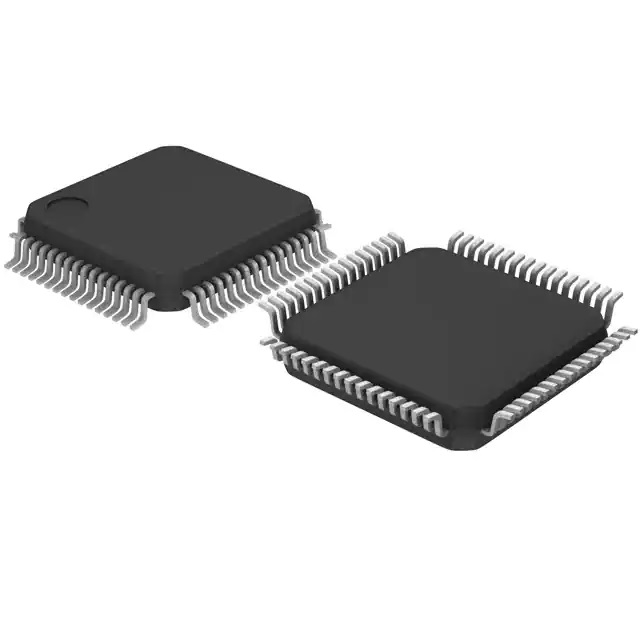
\includegraphics[width=0.3\textwidth]{Figures/64-LQFP}
  \caption[USB Controller]{The USB controller, with 0.5mm between pins}
  \label{fig:USBController}
\end{wrapfigure}
For example, the USB controller chip only has 0.5mm of space between each of it's 64 pins (Figure \ref{fig:USBController}), which would require a breakout board at least 7 times larger than the chip so that each each pin can be easily accessed by hand.
Not to mention the difficulty in wiring up that many pins along with the other related components which would need their own breakout boards either purchased or custom-designed.

Instead, the first board was built out in a piecewise fashion, allowing each section of the board a way to fail without interrupting the rest of the board.
This allows each function of the board to be tested individually and in isolation so that changes could be made incrementally without needing to worry about their integration with the rest of the board.
\todoquestion{This is that tricky sentence}For example, in order to build a system that would allow the board to be powered via USB or an internal battery, as well as charge the battery simultaneously, a complex circuit would have to be built that managed Lithium Polymer (LiPo) batteries which could cause fires if mishandled.
Since power is obviously a critical component of the board, A secondary way of feeding power directly the board was built to bypass all that circuitry in case it fails.
In doing so, the board can still be powered and it's other features can be tested while a fix for that portion of the circuitry is developed for the next iteration.

\begin{figure}[h]
  \centering
  %Height instead of width because the image is rotated
  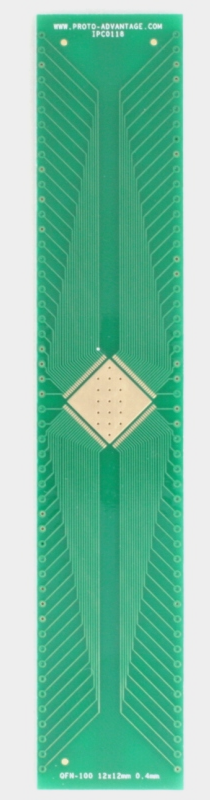
\includegraphics[height=0.9\textwidth,angle=90]{Figures/smt_breakout}
  \captionsetup{width=.8\linewidth}
  \caption[SMD Breakout Board]{A breakout board similar to what would be needer for the USB controller used on the custom PCB}
  \label{fig:smt_breakout}
\end{figure}


\section{Designing the Printed Circuit Board}\label{sec:DesigningThePCB}

Because of the lack of prototyping options discussed in Section \ref{sec:Prototyping}, and ultimate decision to build the board in a way that could safely fail in any way, it became clear that multiple versions of the project were going to need to be designed and produced.
Since the time and budget for this project was limited, the amount of revisioning was minimized by running the circuit by electrical engineering students and professors to catch any potential flaws before the board was manufactured.

\subsection{Power}\label{subsec:DesigningPower}

\begin{figure}[t]
  \centering
  \begin{subfigure}{.5\textwidth}
    \centering
    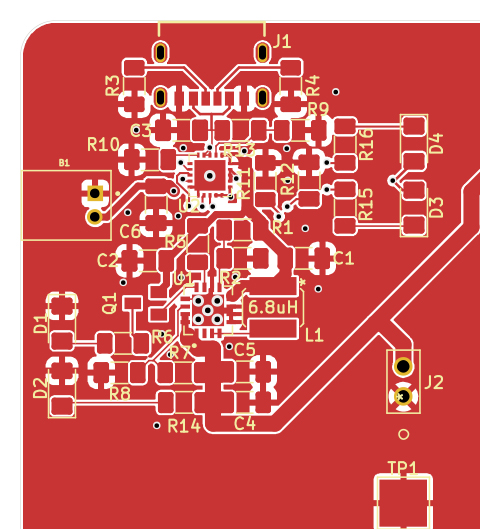
\includegraphics[width=.75\linewidth]{Figures/kicad/close-ups/power-front}
  \end{subfigure}%
  \begin{subfigure}{.5\textwidth}
    \centering
    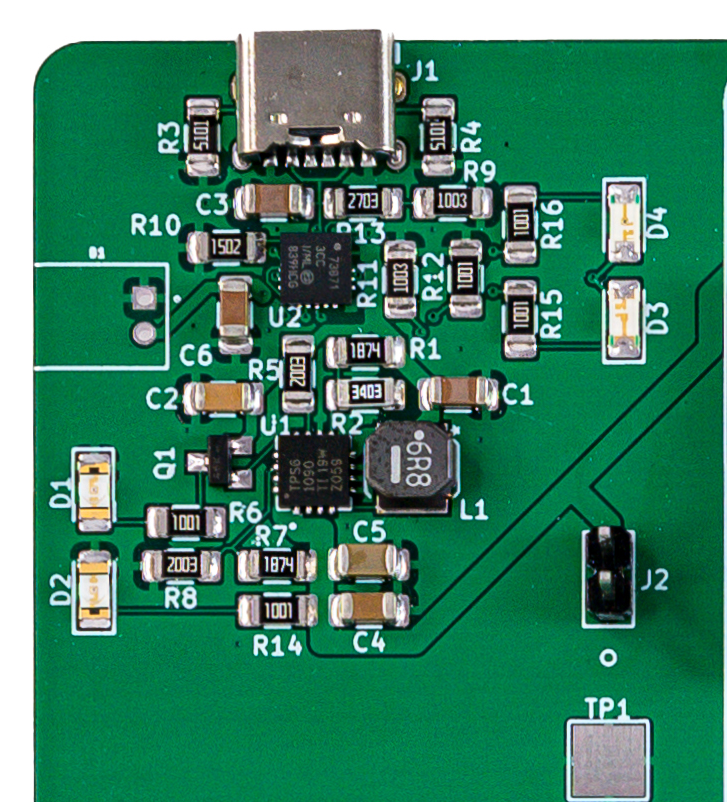
\includegraphics[width=.75\linewidth]{Figures/pcb/crops/power}
  \end{subfigure}
  \caption[PCB Power Circuit]{The front side of the PCB's power circuit}
  \label{fig:PowerCircuit}
\end{figure}

\begin{figure}[b!]
  \centering
  \includegraphics[width=.75\textwidth,page=2]{Figures/kicad/lathrum_thesis_schematic.pdf}
  \caption[Power Schematic]{Schematic layout for the power circuit, including battery management. Expanded in Appendix \ref{app:pcb_schematic_battery}}
  \label{fig:pcb_schematic_battery}
\end{figure}

Development started with arguably the most important part of the board: the power supply (schematic in Figure \ref{fig:pcb_schematic_battery}).
If the CM4 could not receive power, none of the project would work.
A feature of modern devices that has become ubiquitous as much as it has been taken for granted is the ability to charge a battery at the same time it is in use by the device.
This enables the device to be used portably until the battery runs out and then charge the device without needing to stop using it before moving again.
Though it proves to be slightly more complicated than simply connecting the two power supplies.
As seen in Figure \ref{fig:PowerCircuit}, the source of external power, the USB-C port labeled \emph{J1}, has to travel through two integrated circuits before reaching the CM4 through the trace on the right side.
The first chip, \emph{U2}, detailed in Table \ref{tab:SelectedComponents} as \emph{MCP73871-2CCI\_ML}, is used to charge the internal battery attached to the left side of the board through the connector labeled \emph{B1}.
The second chip, \emph{U1}, also detailed in Table \ref{tab:SelectedComponents} as \emph{TPS61090RSAR}, is used to balance the power draw from the USB-C port or the attached battery, favoring the external power when the device is plugged in.
Thankfully, due to the sensitivity of the two chips, their provided datasheets offer specific configurations that they should be designed in to ensure proper functionality.
Although very dense, these blueprints promised individual functionality for each chip, all that was left was connecting them together.
The two of these chips must work in tandem for power to be successfully delivered to the CM4, if either failed, none of the other parts of the board could be tested.
In the event this happened, a secondary method of powering the board directly was added in the form of the generic two-pin header \emph{J2}.
These two pins are simply 5v input and ground through-hole pins that bypass all the power circuitry just described.
Once the CM4 could be powered, the rest of the I/O could be designed.

\subsection{USB}\label{subsec:DesigningUSB}

\begin{figure}[t]
  \centering
  \begin{subfigure}{.5\textwidth}
    \centering
    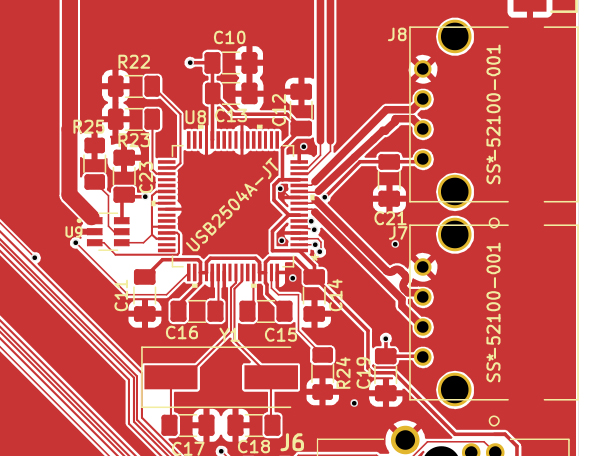
\includegraphics[width=.75\linewidth]{Figures/kicad/close-ups/usb-front}
  \end{subfigure}%
  \begin{subfigure}{.5\textwidth}
    \centering
    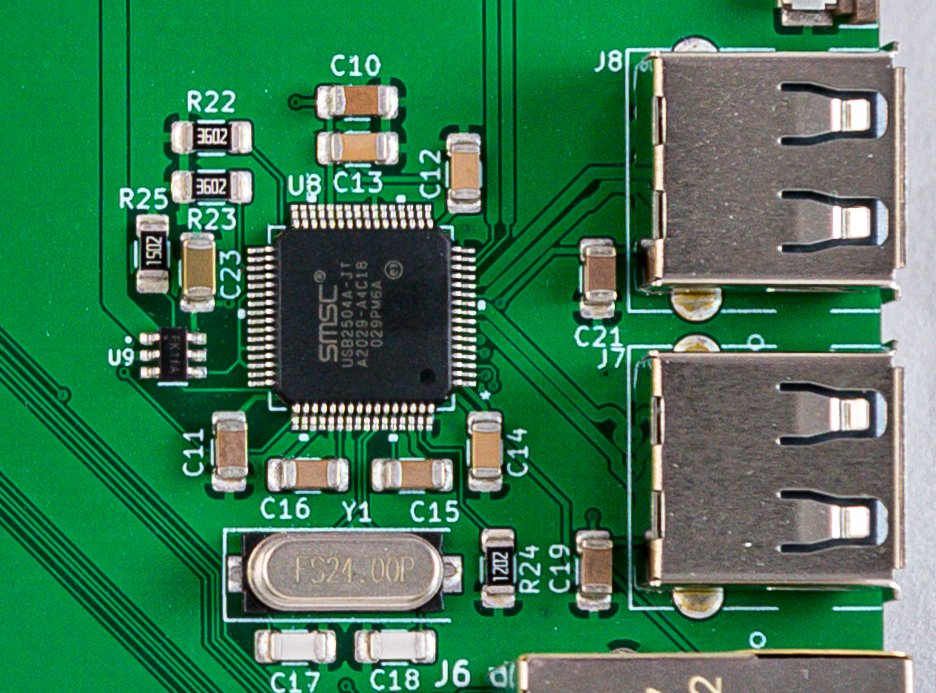
\includegraphics[width=.75\linewidth]{Figures/pcb/crops/usb}
  \end{subfigure}
  \caption[PCB USB Circuit]{The front side of the PCB's USB circuit}
  \label{fig:USBCircuit}
\end{figure}

\begin{figure}[b!]
  \centering
  \includegraphics[width=.75\textwidth,page=4]{Figures/kicad/lathrum_thesis_schematic.pdf}
  \caption[USB Schematic]{Schematic layout for the USB hub and ports. Expanded in Appendix \ref{app:pcb_schematic_usb}}
  \label{fig:pcb_schematic_usb}
\end{figure}

The next prominent circuit on the board is the section that controls the USB ports.
As seen in Figure \ref{fig:USBCircuit} (schematic in Figure \ref{fig:pcb_schematic_usb}), the dense circuit is mostly comprised of the USB controller chip, \emph{U8}, it's associated components, and the four USB ports, two of which are pictured as \emph{J7} and \emph{J8}.
Similarly to the power circuit, the USB controller chip is a very sensitive component that must be arranged in relation to other components in a certain way in order to ensure it will function properly.
This includes surrounding the chip with numerous capacitors to normalize any small power fluctuations, using a specific load balancing power distribution switch (\emph{U9}), and an oscillating crystal to provide a stable clock for the chip.
The chip connects to each of the four downstream USB ports and handles all of the digital signal processing before sending the data to the upstream CM4.

\subsection{HDMI}\label{subsec:DesigningHDMI}

\begin{figure}[t]
  \centering
  \begin{subfigure}{.33\textwidth}
    \centering
    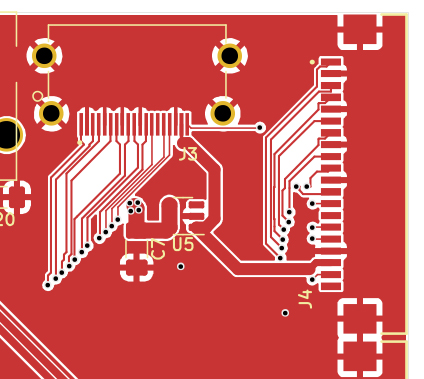
\includegraphics[width=1\linewidth]{Figures/kicad/close-ups/hdmi-front}
    \caption{The front side of the PCB}
    \label{fig:HDMICircuitFront}
  \end{subfigure}%
  \begin{subfigure}{.33\textwidth}
    \centering
    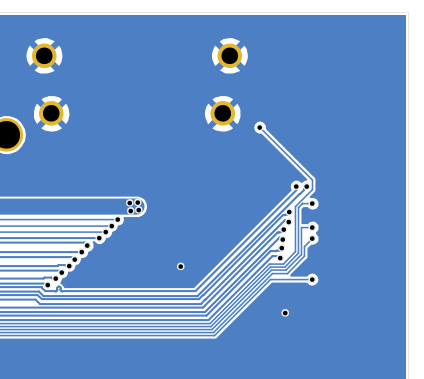
\includegraphics[width=1\linewidth]{Figures/kicad/close-ups/hdmi-back}
    \caption{The back side of the PCB}
    \label{fig:HDMICircuitBack}
  \end{subfigure}%
  \begin{subfigure}{.33\textwidth}
    \centering
    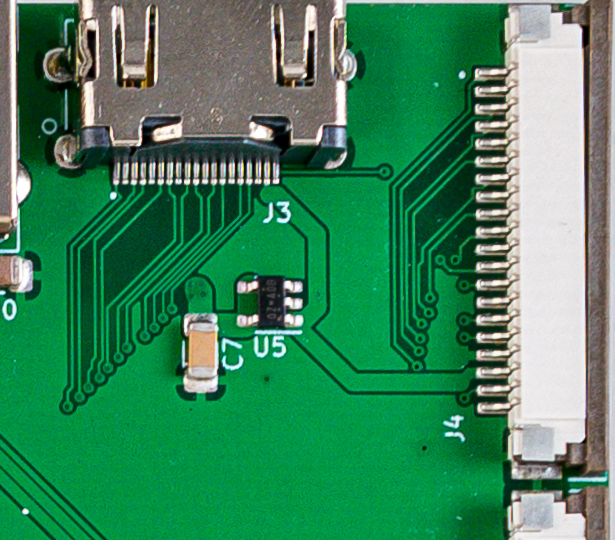
\includegraphics[width=1\linewidth]{Figures/pcb/crops/hdmi}
    \caption{The physical PCB}
    \label{fig:HDMICircuitReal}
  \end{subfigure}
  \caption{The PCB's HDMI circuit}
  \label{fig:HDMICircuit}
\end{figure}

% While this is the image for the CM4 section, it makes sense to put it here
\begin{figure}[b!]
  \centering
  \begin{subfigure}{.33\textwidth}
    \centering
    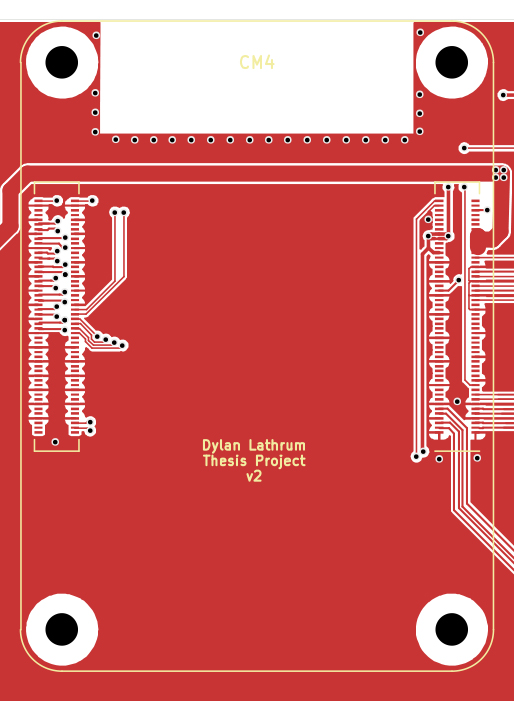
\includegraphics[width=.95\linewidth]{Figures/kicad/close-ups/cm4-front}
    \caption{The front side of the PCB}
    \label{fig:CM4CircuitFront}
  \end{subfigure}%
  \begin{subfigure}{.33\textwidth}
    \centering
    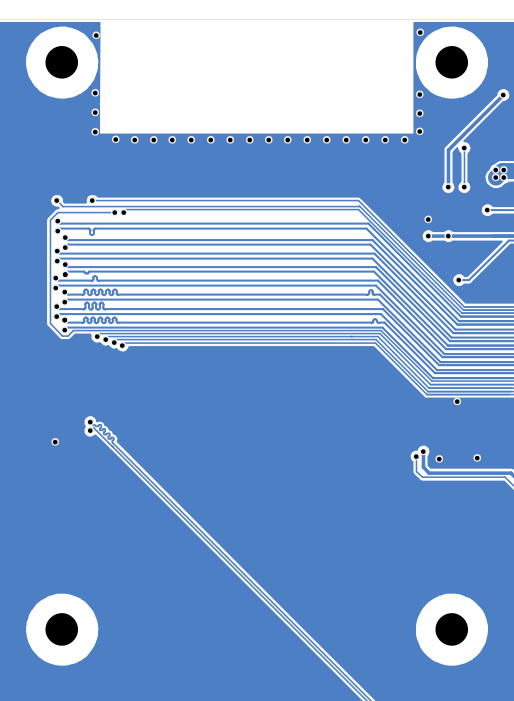
\includegraphics[width=.95\linewidth]{Figures/kicad/close-ups/cm4-back}
    \caption{The back side of the PCB}
    \label{fig:CM4CircuitBack}
  \end{subfigure}%
  \begin{subfigure}{.33\textwidth}
    \centering
    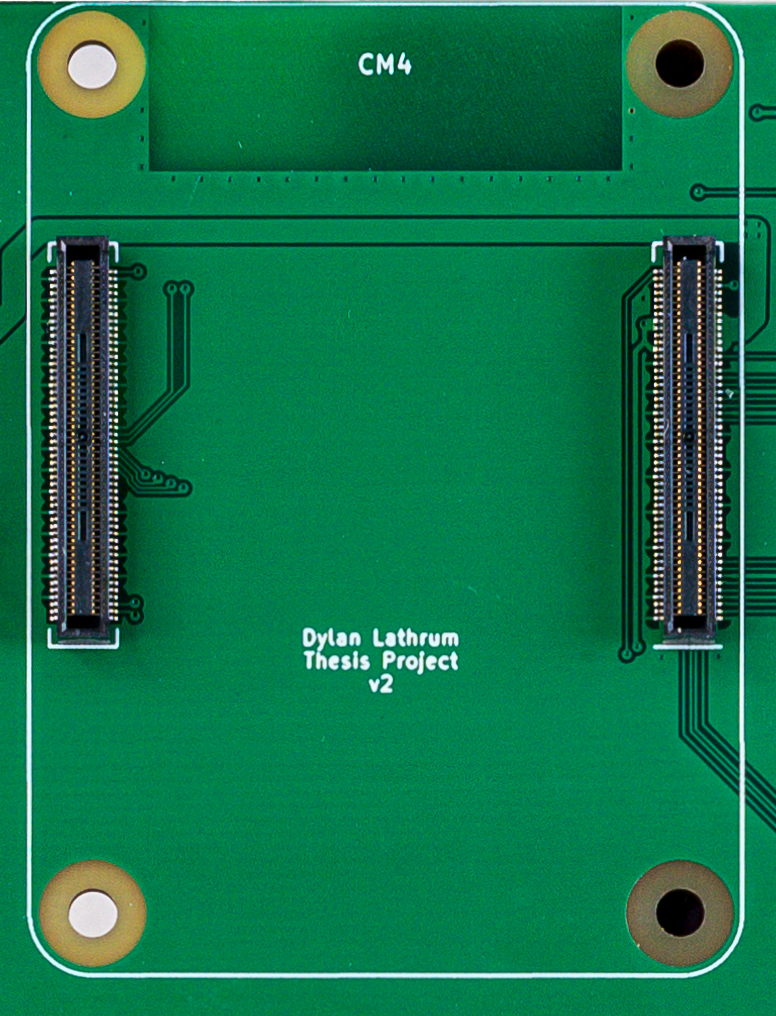
\includegraphics[width=.95\linewidth]{Figures/pcb/crops/cm4}
    \caption{The physical PCB}
    \label{fig:CM4CircuitReal}
  \end{subfigure}
  \caption{The circuitry surrounding the CM4's two mezzanine connectors}
  \label{fig:CM4Circuit}
\end{figure}

Another vital part of the board is the two HDMI ports provided by the device.
Thankfully, unlike the USB ports, HDMI ports send information in only one direction, so an extra chip is not necessary to handle the data as an intermediary.
All that is necessary is to connect the two HDMI ports to the CM4 in the right order and the device will be able to output the rendered video to a display.
Because this device is intended to be a standalone machine, it makes sense to have essential components like a screen integrated as part of the design.
The only issue with simply attaching an HDMI cable inside of the device is that the ports are relatively bulky and inflexible, meaning that another solution must be created to fit in the tight space.
This is accomplished with the Flat Flexible Cable Connector, seen on the right side of Figure \ref{fig:HDMICircuitFront} as \emph{J4}.
Flat Flexible Cables (FFC) are generic bendable cables that can be used in tight spaces.
Even though their connectors are completely generic, meaning that they have no set pinout, it is possible to use them given that the receiving screen will take in the FFC in the same order as a HDMI cable.
Using this knowledge, an internal FFC can be wired for the device's primary screen, while a second traditional HDMI port can be exposed to the user in case they want to use an external monitor.
This, along with the FFC used for one of the four USB ports, allows a screen to be hooked up to the CM4 internally without needing to expose anything to the user.

\subsection{CM4 and Miscellaneous}\label{subsec:DesigningCM4}

\begin{figure}[t!]
  \centering
  \includegraphics[width=.75\textwidth,page=3]{Figures/kicad/lathrum_thesis_schematic.pdf}
  \caption[USB Schematic]{Schematic layout for interfacing with the Compute Module 4. Expanded in Appendix \ref{app:pcb_schematic_cm4}}
  \label{fig:pcb_schematic_cm4}
\end{figure}

Finally, everything must connect to the CM4.
Figure \ref{fig:CM4Circuit} shows the the two mezzanine connectors the CM4 uses to communicate with the rest of the PCB (schematic in Figure \ref{fig:pcb_schematic_cm4}).
Remember that there is only 0.04mm of space in between each of the pins, leaving very little space to route the traces where they need to go.
The first thing to notice is the large stretch of traces on the back side of the board coming from the HDMI ports.
Because most of the traces come in positive and negative pairs, called differential pairs, the two tracks must be roughly the same length as each other.
This is because as data is transmitted across the pair of tracks, they need to arrive at their destination at the same time based on the physical distance the signals need to cover.
Since the speed of electricity is constant throughout the PCB board, the traces may need to wind back and forth so that the lengths of the positive and negative tracks are equal.
Also note the blank area surrounded by vias at the top of Figure \ref{fig:CM4Circuit}.
This is where the WiFi and Bluetooth antennas are located on the CM4 board.
By removing the copper pour from this area on the PCB board and stitching the perimeter with vias, it prevents the board from acting like another antenna and interfering with the signals being sent to and from the CM4.
Finally, each of the other components are connected to the CM4 board in the same manner as described throughout this chapter, such as the Ethernet adapter, the SD card reader, and remaining ports.
\todoadvisor{Why are those components not described in the same way as power/USB/etc.?}\todoquestion{The Ethernet port is hooked directly into the CM4 connector with nothing interested except that they are also differential pairs, as described in the HDMI section. I suppose they could be explained fully, but I worry that it wouldn't add any useful information.}
See Appendices \ref{AppendixA} and \ref{AppendixB} for further information.


\section{Manufacturing the Circuit Board}\label{sec:ManufacturingThePCB}

\begin{figure}[t]
  \centering
  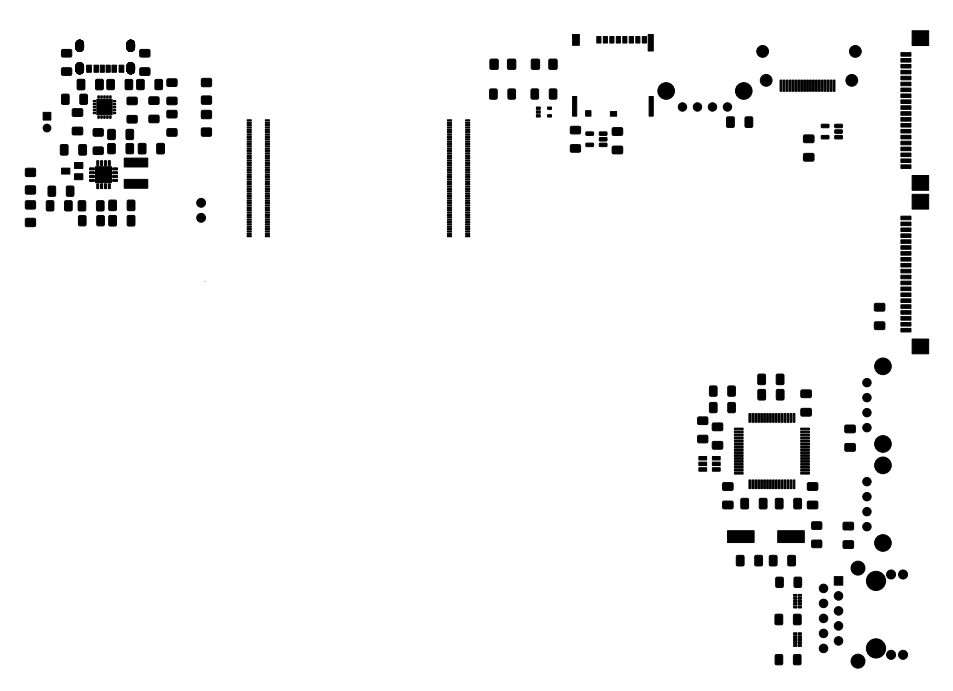
\includegraphics[width=0.5\textwidth]{Figures/kicad/close-ups/stencil}
  \caption[PCB Stencil]{The PCB's stencil. Areas colored black are where solder paste is applied to solder SMD parts to the board}
  \label{fig:PCBStencil}
\end{figure}

\todo[inline]{Insert pictures of PCB. Thinking at least one showing the flaws of the first board, another of the completed board}

Once the board's design has been completed and checked against all electrical, functional, and manufacturing constraints, the Printed Circuit Board can be produced.
The first step in fabrication is to print the actual PCB.
While ASU offers a basic printing service for use in classes and academic projects, the requirements of this board, specifically the tiny traces and pads required for the CM4's mezzanine connectors (pictured in Figure \ref{fig:rpi_cm4_mezzanine}), are outside of the printer's capabilities.
Instead, by recommendation of a professor, the printing was done through an external company that provides quick turnaround and low costs for printing PCBs \cite{jlcpcb}.
A set of five boards was ordered, allowing for multiple boards to be assembled in case of error, as well as a stencil.
A PCB stencil is a thin sheet of metal with holes cut in it that line up with the pads on the PCB board.
This enables the easy application of solder paste onto all of the pads on the board as once, including the difficulty small pads of the CM4's mezzanine connectors.
While the PCB was being printed, all of the parts found in the Bill of Materials (found in Appendix \ref{AppendixB}) were ordered from sites such as Digi-Key and Mouser \cite{digikey,mouser}.
In order to account for the production of multiple prototype boards and the possibility of broken parts, enough parts were ordered to produce five complete boards.

\subsection{First Attempt}\label{subsec:Manufacturing1}

Once the PCB and it's component parts arrived, the board could be assembled.
The first board was assembled by hand using the PCB stencil and a handheld heat gun.
The stencil, shown as an image in Figure \ref{fig:PCBStencil}, is used by securing it the PCB board so that the holes line up with the pads, and spreading solder paste across it allowing the paste to cover the exposed pads through the holes.
The stencil was then removed, and each of the surface mounted components were then placed onto the board using a set of tweezers.
For tricky parts such as the CM4's mezzanine connectors and other small parts with the pads below the component itself, a microscope was used to assist in lining up the pads with the components.
Once the parts were placed, a heat gun was used to melt the solder paste and fuse the components to the board.
Following the SMDs, the through-hole components, such as the ports lining the side of the board, were then placed and soldered using a hand-held soldering iron.

\begin{figure}[t]
  \centering
  \includegraphics[width=0.4\textwidth]{Figures/pcb/handmade_mezzanine.JPG}
  \caption[Hand-soldered mezzanine connector]{The leftovers of the broken-off mezzanine connector from the hand-soldered first board. Notice the exposed copper and warped pads.}
  \label{fig:brokenmezzanine}
\end{figure}

The first board ran into two issues that prevented it from working.
Firstly, due to improper use of the heat gun, most of the LEDs had popped, resulting in all hardware-level diagnostic indicators being inoperable.
Secondly, the CM4 connectors were not properly connected to the board, and in an attempt to repair it, the connector components were irreparably damaged and the board itself was damaged slightly, seen in Figure \ref{fig:brokenmezzanine}.
Instead of attempting to assemble another board by hand, a local third-party company was contacted to assemble the board professionally.
After delivering the board, stencil, and parts, the second board was assembled.

\subsection{Second Attempt}\label{subsec:Manufacturing2}

\begin{figure}[b]
  \centering
  \begin{subfigure}{.5\textwidth}
    \centering
    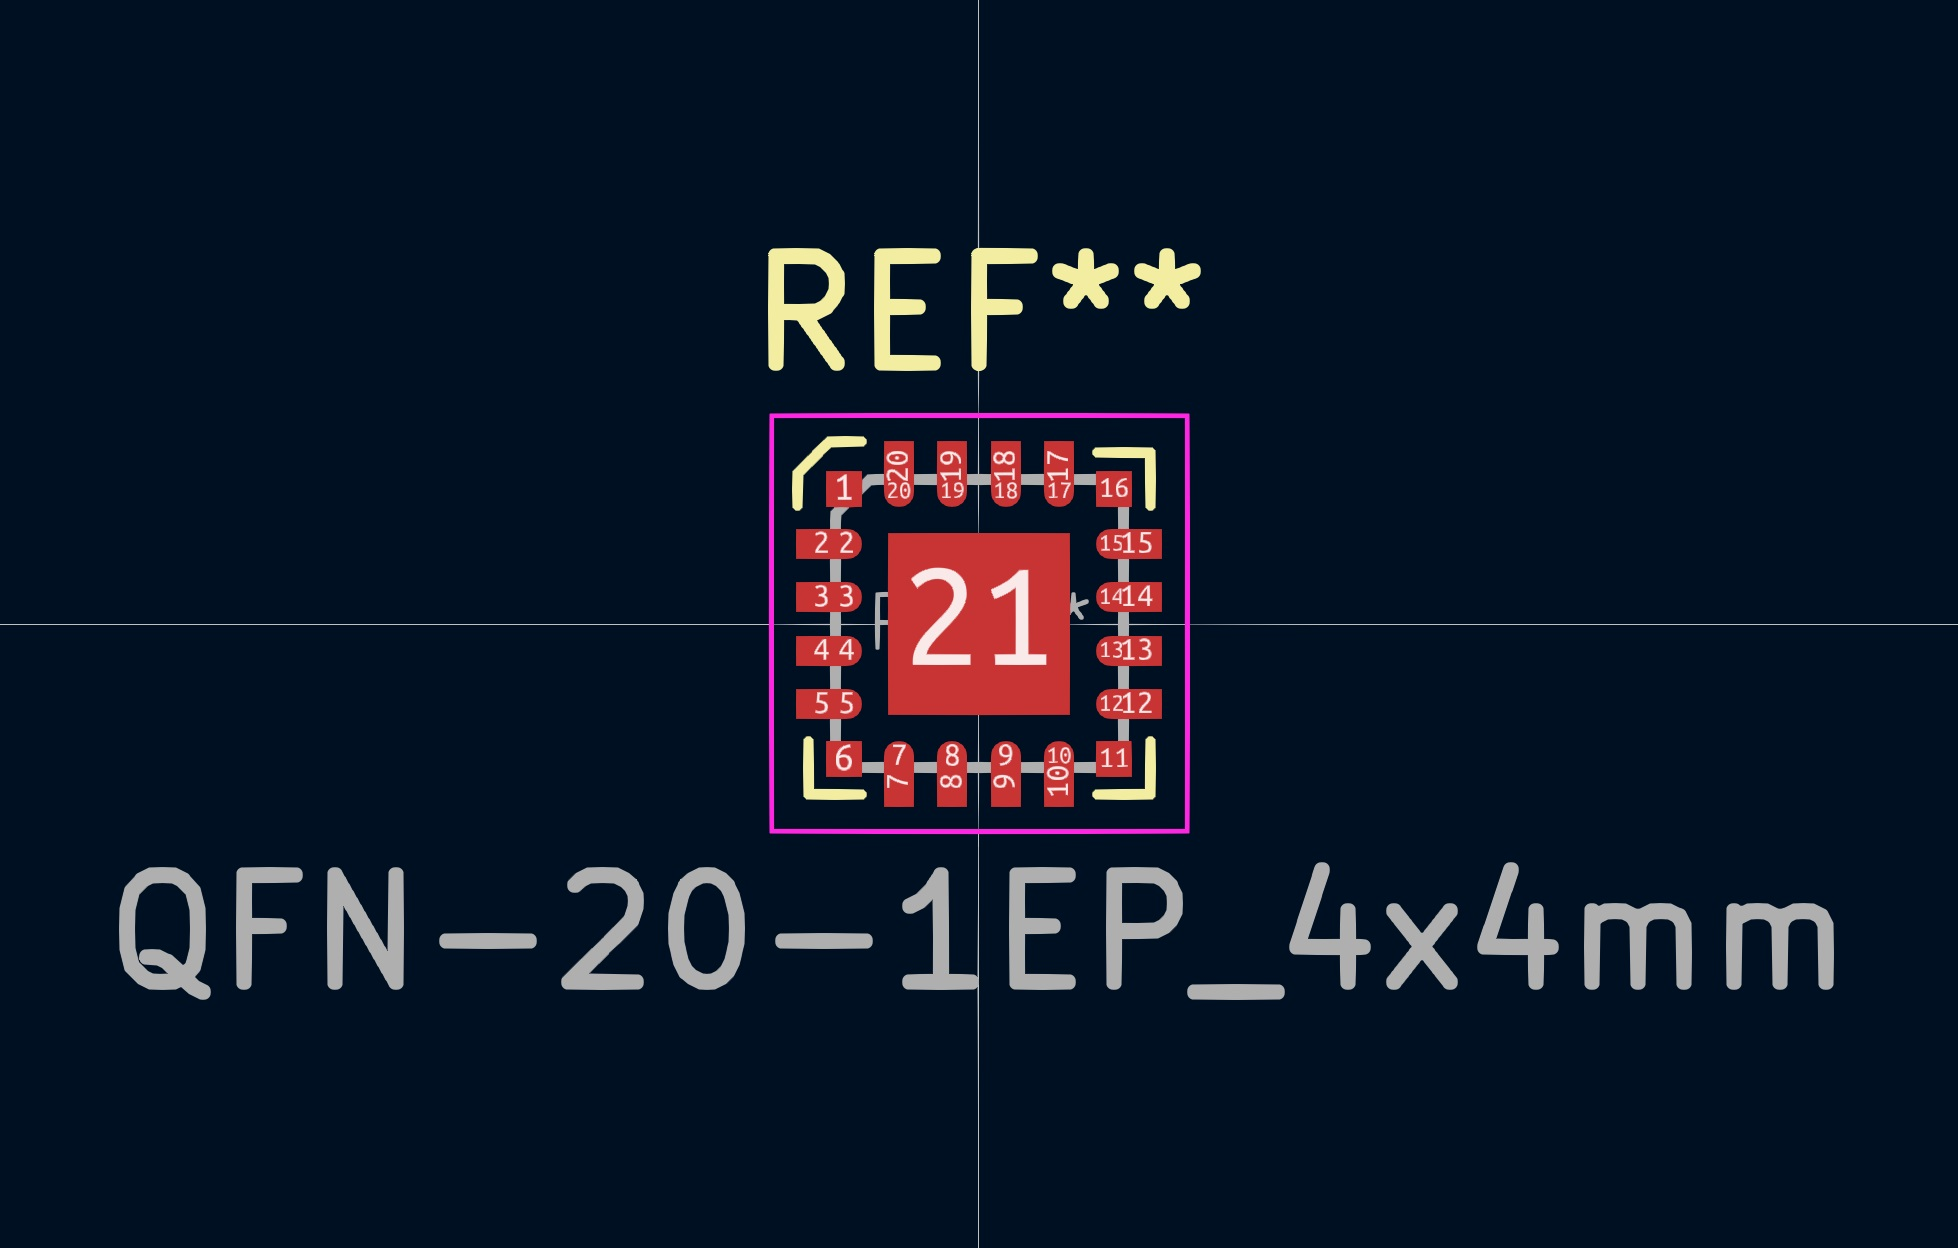
\includegraphics[width=.8\linewidth]{Figures/kicad/QFN-20-1EP_4x4mm}
    \caption{\emph{QFN-20-1EP\_4x4mm}}
    \label{fig:FootprintQFN204x4_Original}
  \end{subfigure}%
  \begin{subfigure}{.5\textwidth}
    \centering
    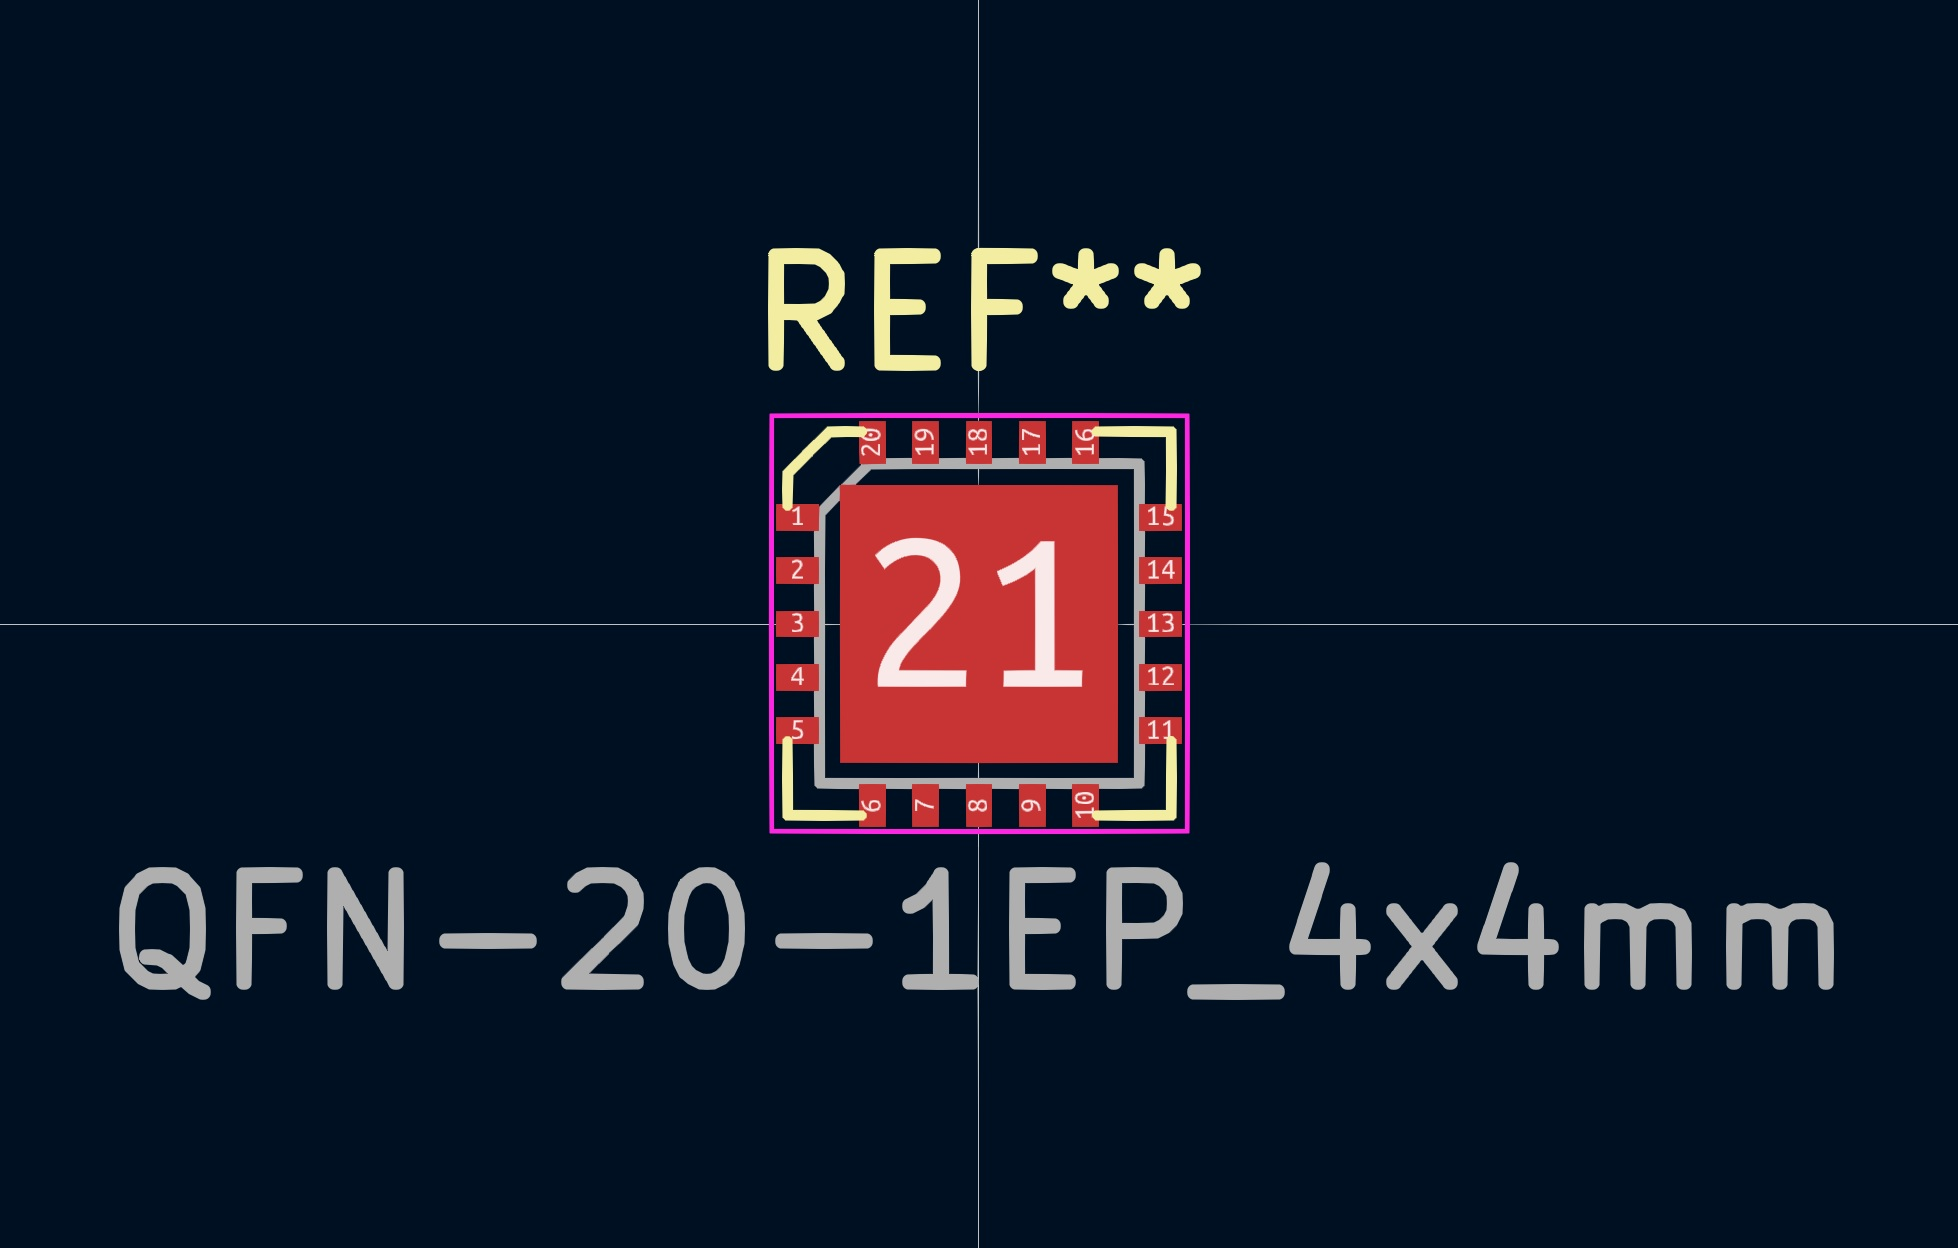
\includegraphics[width=.8\linewidth]{Figures/kicad/QFN-20-1EP_4x4mm_RevA}
    \caption{\emph{QFN-20-1EP\_4x4mm\_RevA}}
    \label{fig:FootprintQFN204x4_RevA}
  \end{subfigure}
  \caption[Two versions of the QFN-20-1EP\_4x4mm package]{The two footprints for components with the \emph{QFN-20-1EP\_4x4mm} package. The original footprint is shown in Figure \ref{fig:FootprintQFN204x4_Original}, while the revised footprint is shown in Figure \ref{fig:FootprintQFN204x4_RevA}}
  \label{fig:FootprintQFN204x4}
\end{figure}

The second board was assembled mostly successfully, and allowed the first stage of testing to begin.
The only issue apart from some ports being too close together with real-world cables was one component having the wrong footprint on the board.
Unfortunately, the component \emph{U2 (MCP73871-2CCI\_ML)}, is described as using the \emph{QFN-20-1EP\_4x4mm} footprint in it's datasheet\todoquestion{Does this need to be cited? Can you cite a datasheet like this?}, but actually uses a revised version of the footprint, shown in Figure \ref{fig:FootprintQFN204x4}.
This discrepancy meant that that component could not be soldered, and it's associated circuit would not function properly.
In this case, the component was a part of the battery charging circuit, causing the entire primary power supply to be unusable.
Thankfully, as described in Section \ref{sec:Prototyping}, the secondary method of powering the board could be used to test the remaining features of the board.
After making the necessary fixes, a second round of five PCB boards and a stencil was ordered.
Because there was still enough components to assemble three more boards, and no components needed to be changed, no more components were ordered at this stage.
Once the boards were delivered, the revised board was again sent to be professionally assembled.

\subsection{Third Attempt}\label{subsec:Manufacturing3}

\begin{figure}[t]
  \centering
  \includegraphics[width=0.8\textwidth]{Figures/pcb/crops/final}
  \caption[Assembled PCB]{The assembled PCB}
  \label{fig:AssembledPCB}
\end{figure}

Once the third board was assembled, the board could be tested in full.
While each part of the board was at least partially functional, there were still issues preventing it from working completely.
In particular, USB devices plugged into any of the ports on the board were able to receive power from the board but were unable to transfer data in either direction.
\todo[inline]{I am currently going through and diagnosing this issue}